\section{Ainul Filiani (1174073)}
\subsection{Menulis Shapefile dengan PySHP}
\begin{enumerate}
	\item Nomor 1
	\lstinputlisting{src/tugas2/1174073/No1.py}
	\begin{figure}[H]
		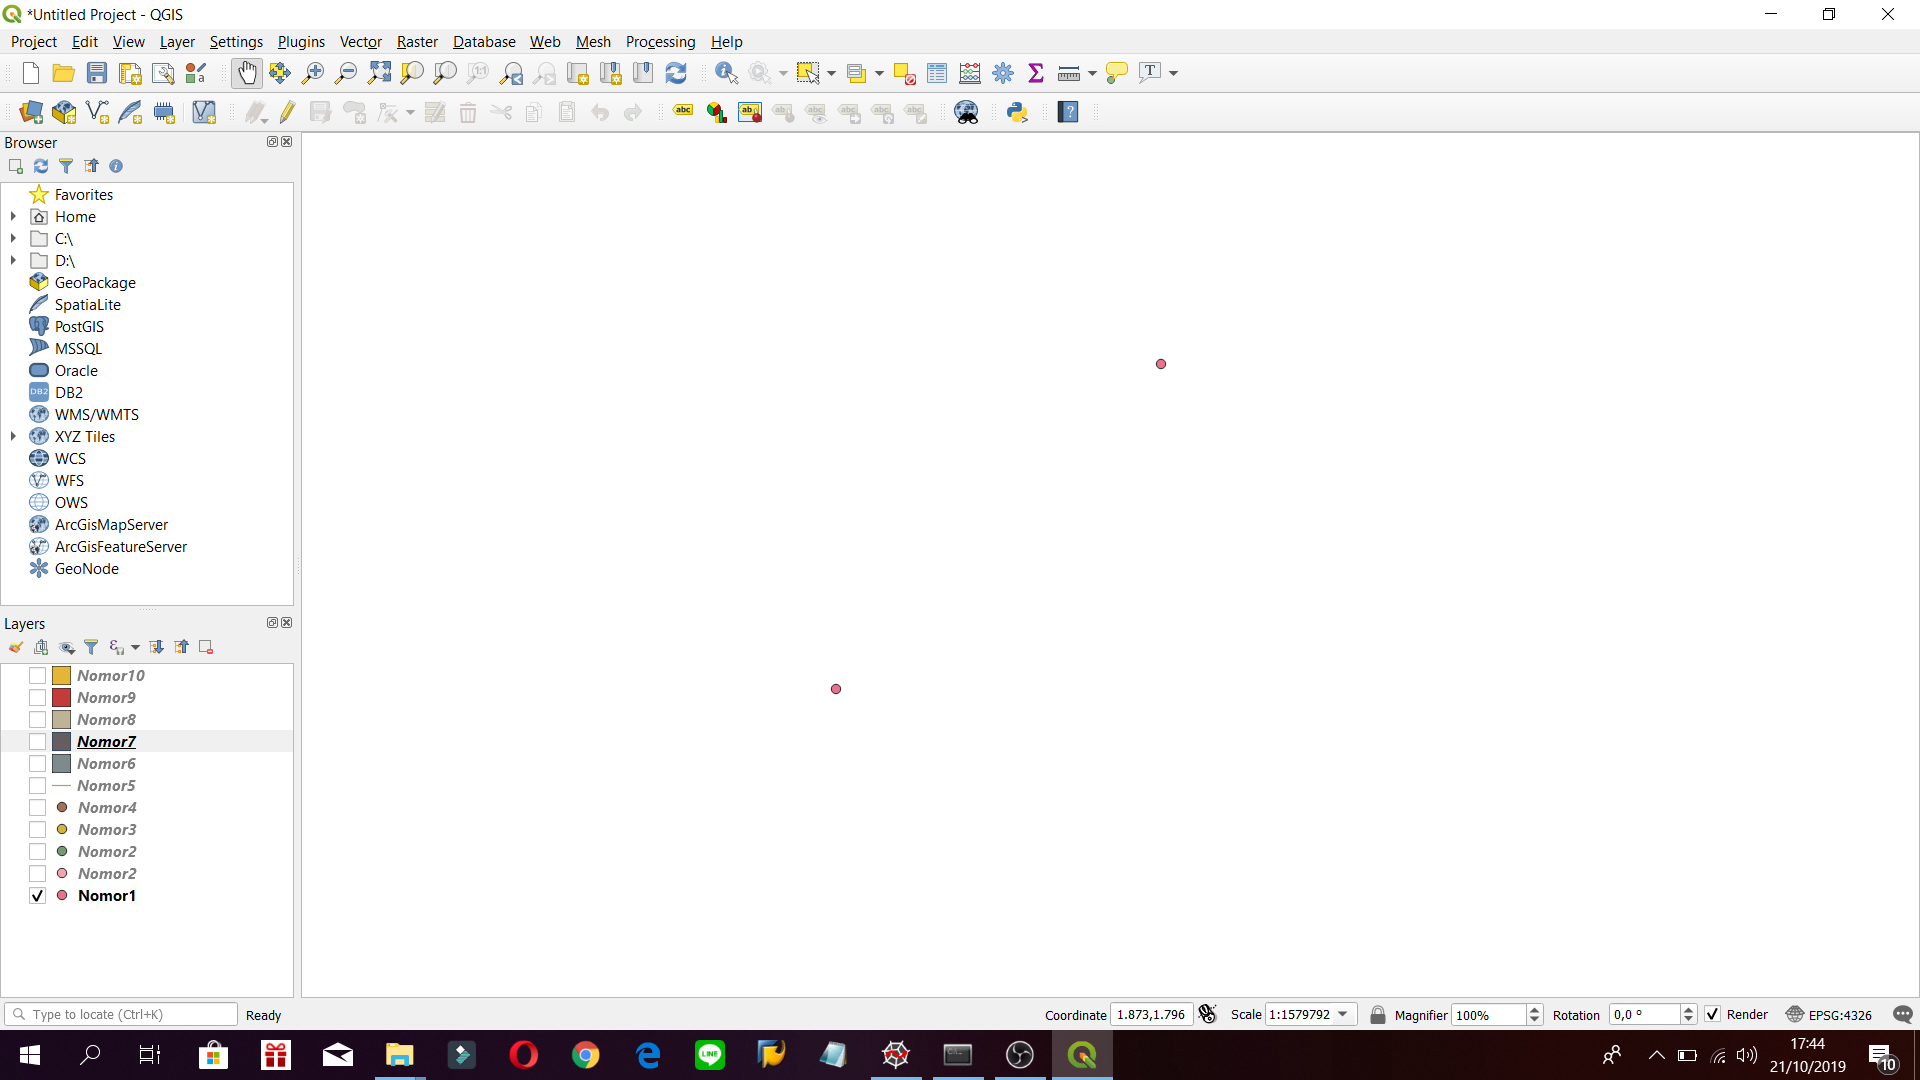
\includegraphics[width=6cm]{figures/Tugas2/1174073/No1.png}
		\centering
		\caption{Point (Titik)}
	\end{figure}
	\item Nomor 2
	\lstinputlisting{src/tugas2/1174073/No2.py}
	\begin{figure}[H]
		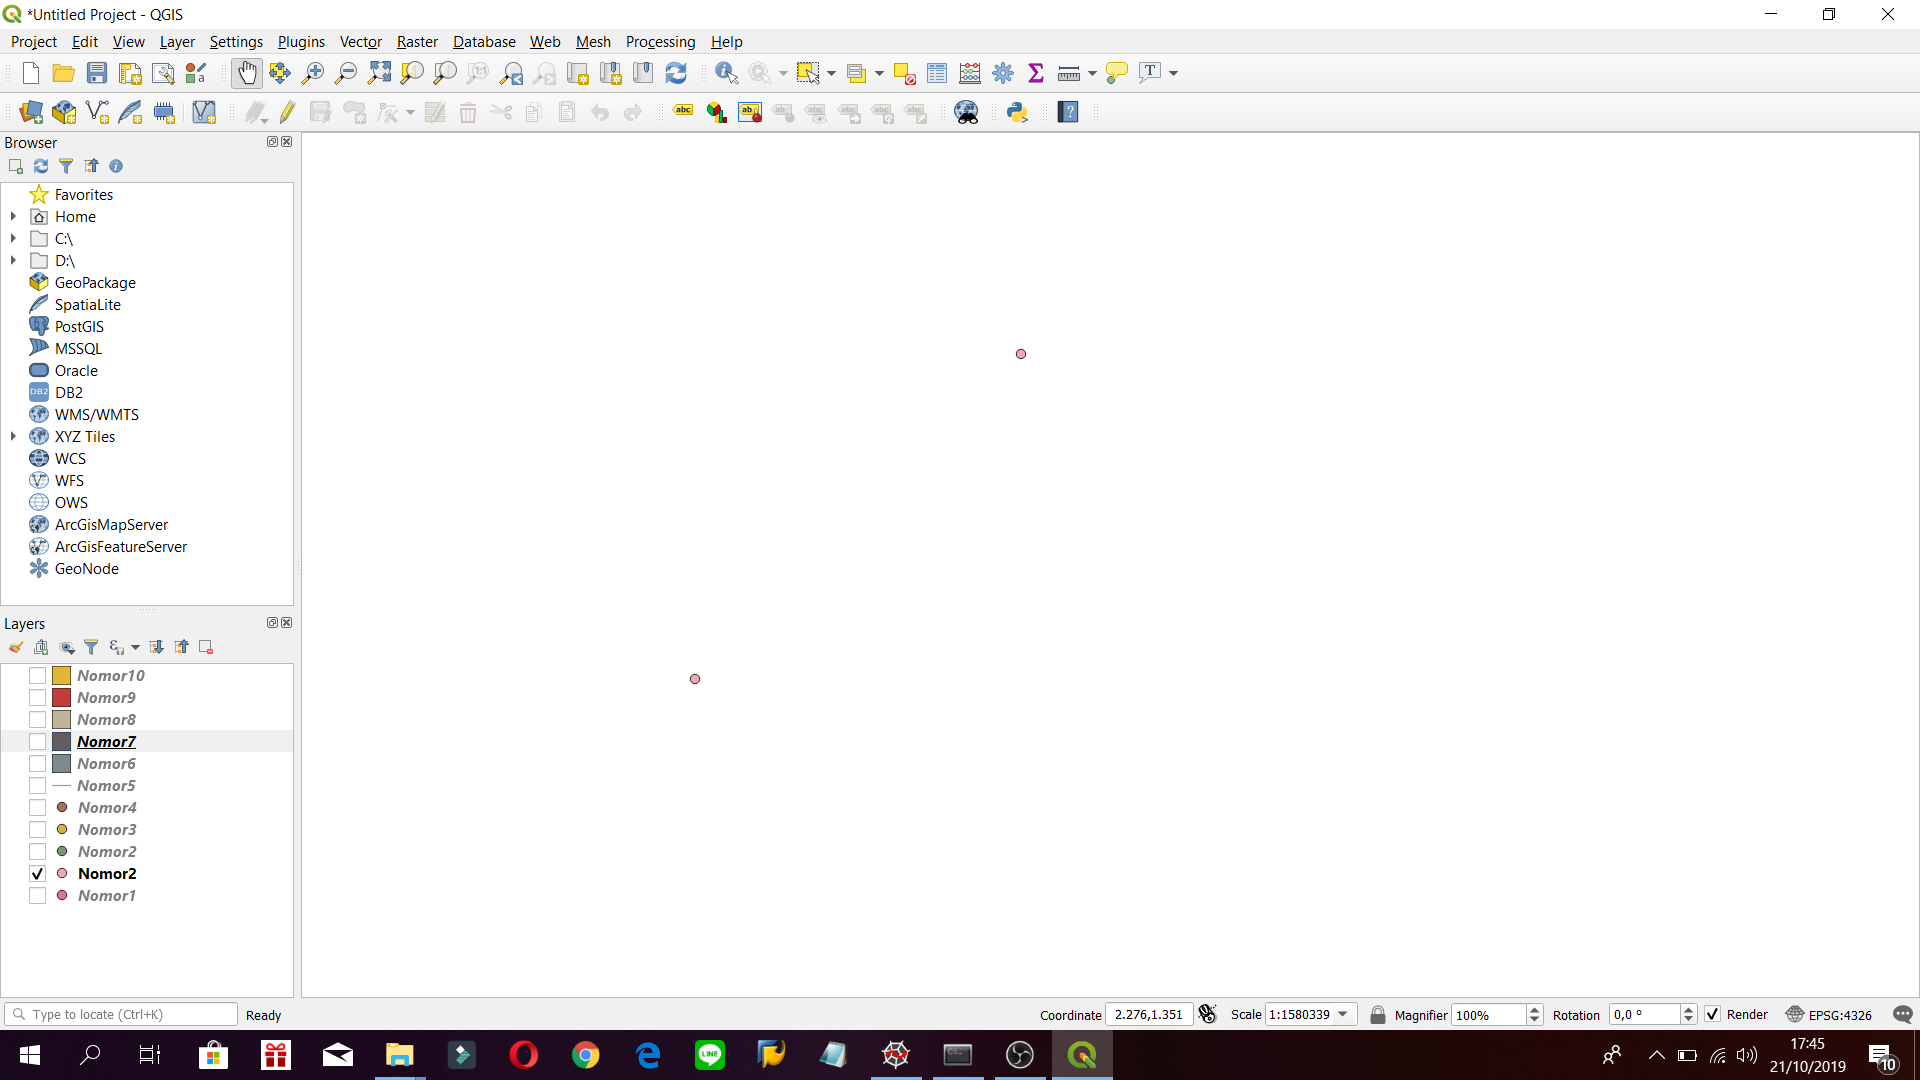
\includegraphics[width=6cm]{figures/Tugas2/1174073/No2.png}
		\centering
		\caption{Point (Titik)}
	\end{figure}
	\item Nomor 3
	\lstinputlisting{src/tugas2/1174073/No3.py}
	\begin{figure}[H]
		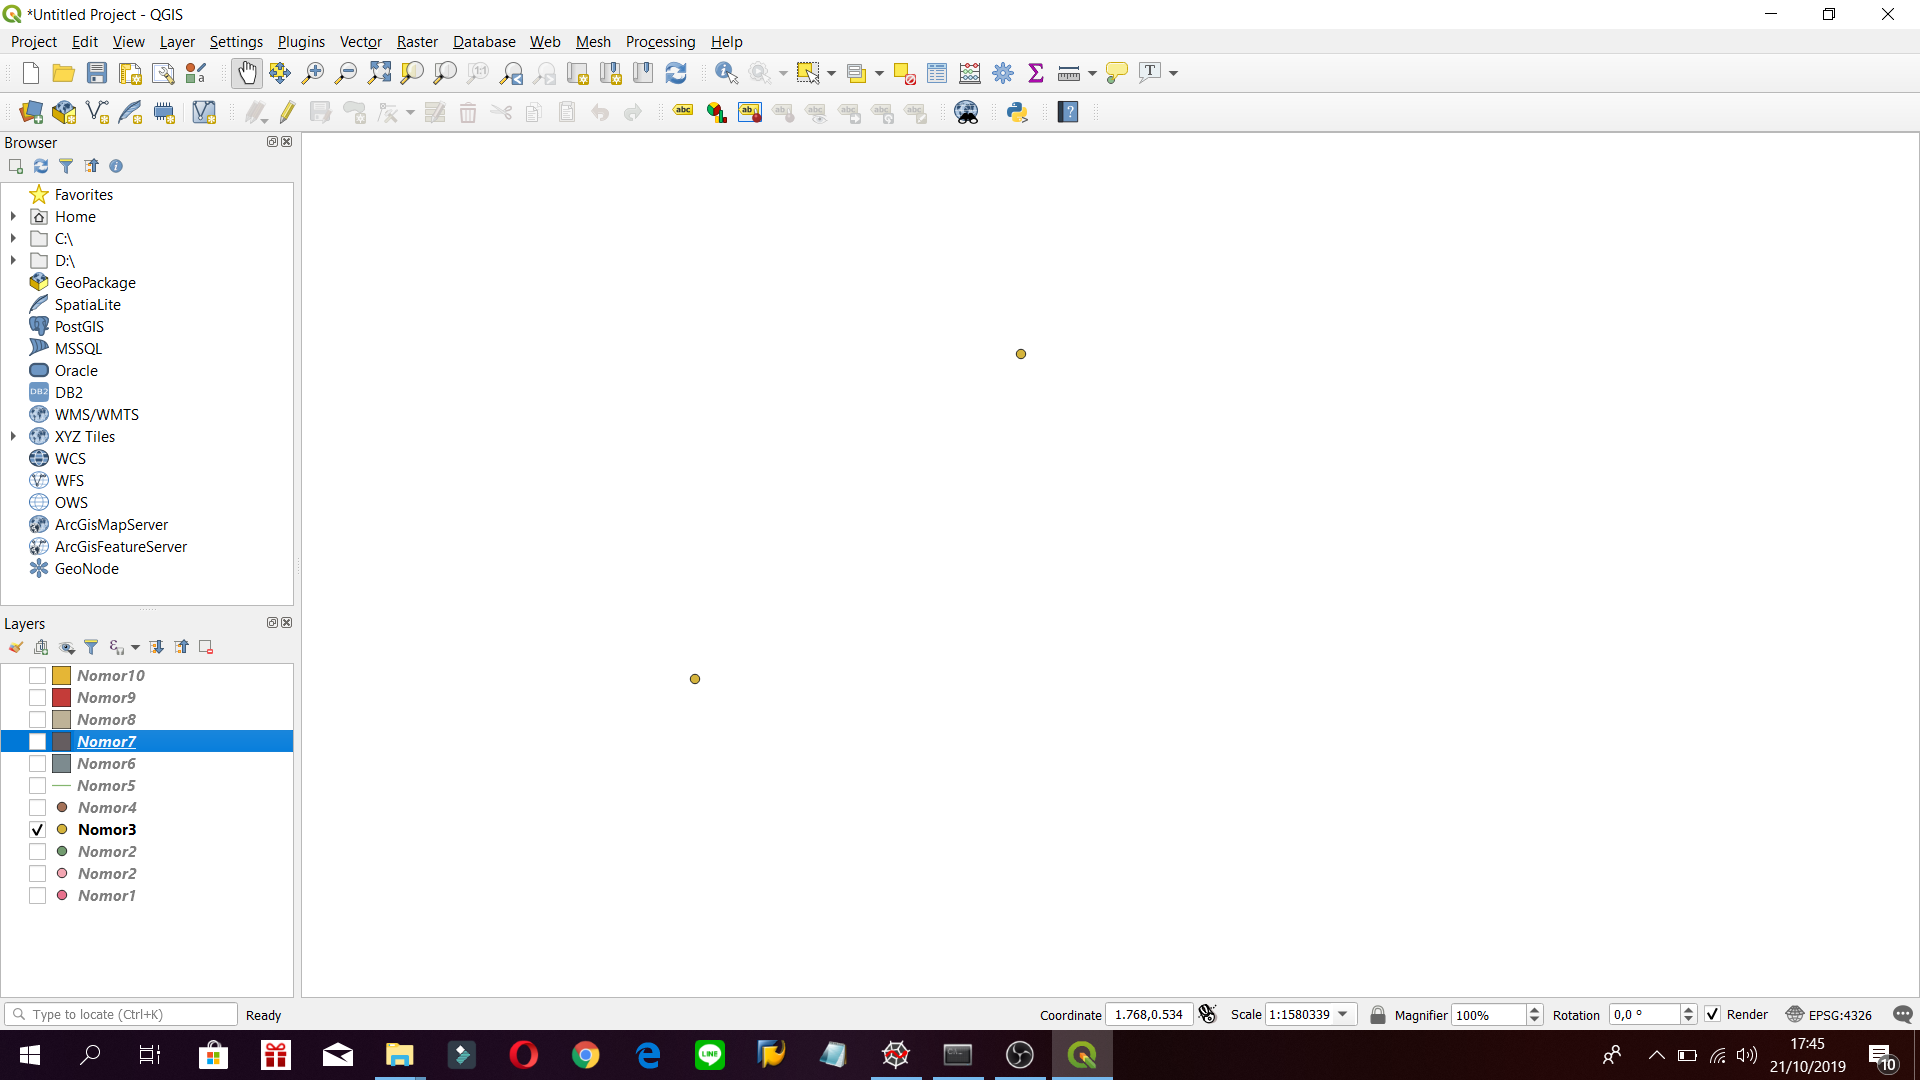
\includegraphics[width=6cm]{figures/Tugas2/1174073/No3.png}
		\centering
		\caption{Point (Titik)}
	\end{figure}
	\item Nomor 4
	\lstinputlisting{src/tugas2/1174073/No4.py}
	\begin{figure}[H]
		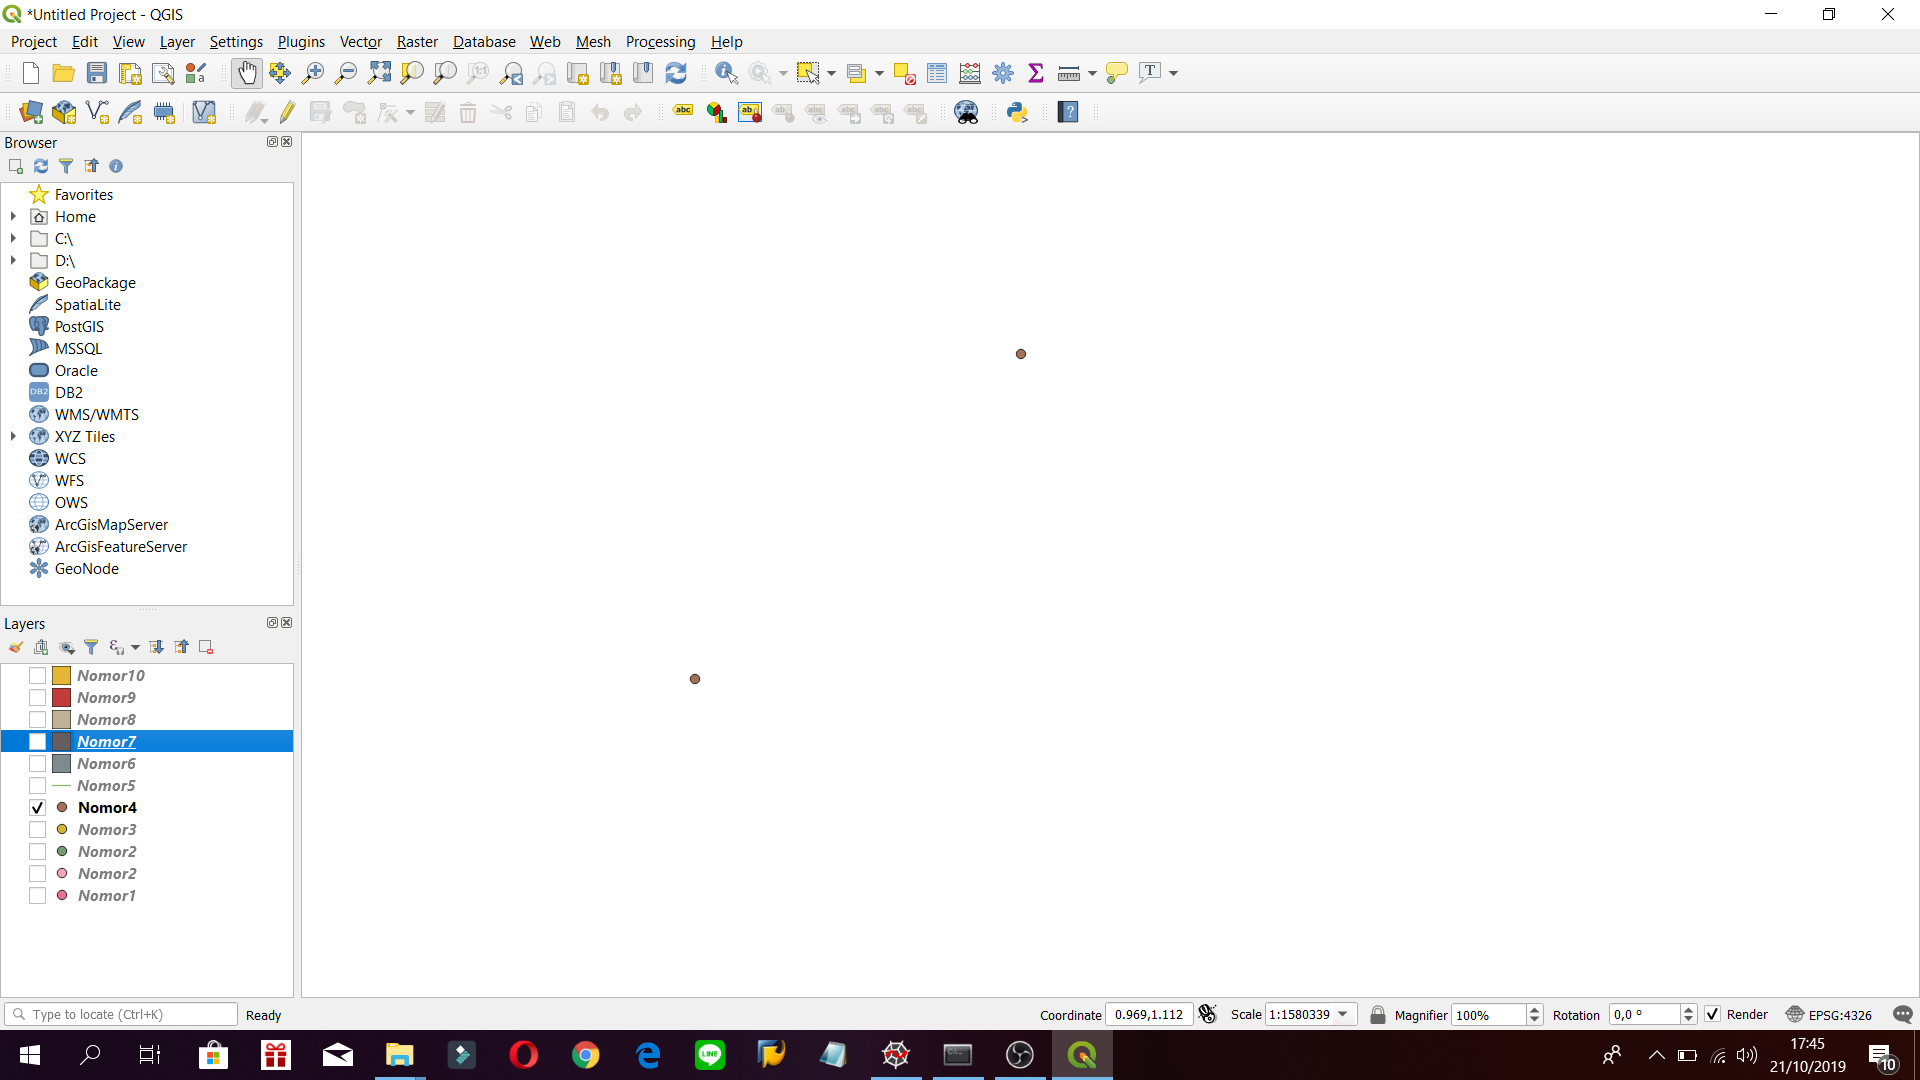
\includegraphics[width=6cm]{figures/Tugas2/1174073/No4.png}
		\centering
		\caption{Point (Titik)}
	\end{figure}
	\item Nomor 5
	\lstinputlisting{src/tugas2/1174073/No5.py}
	\begin{figure}[H]
		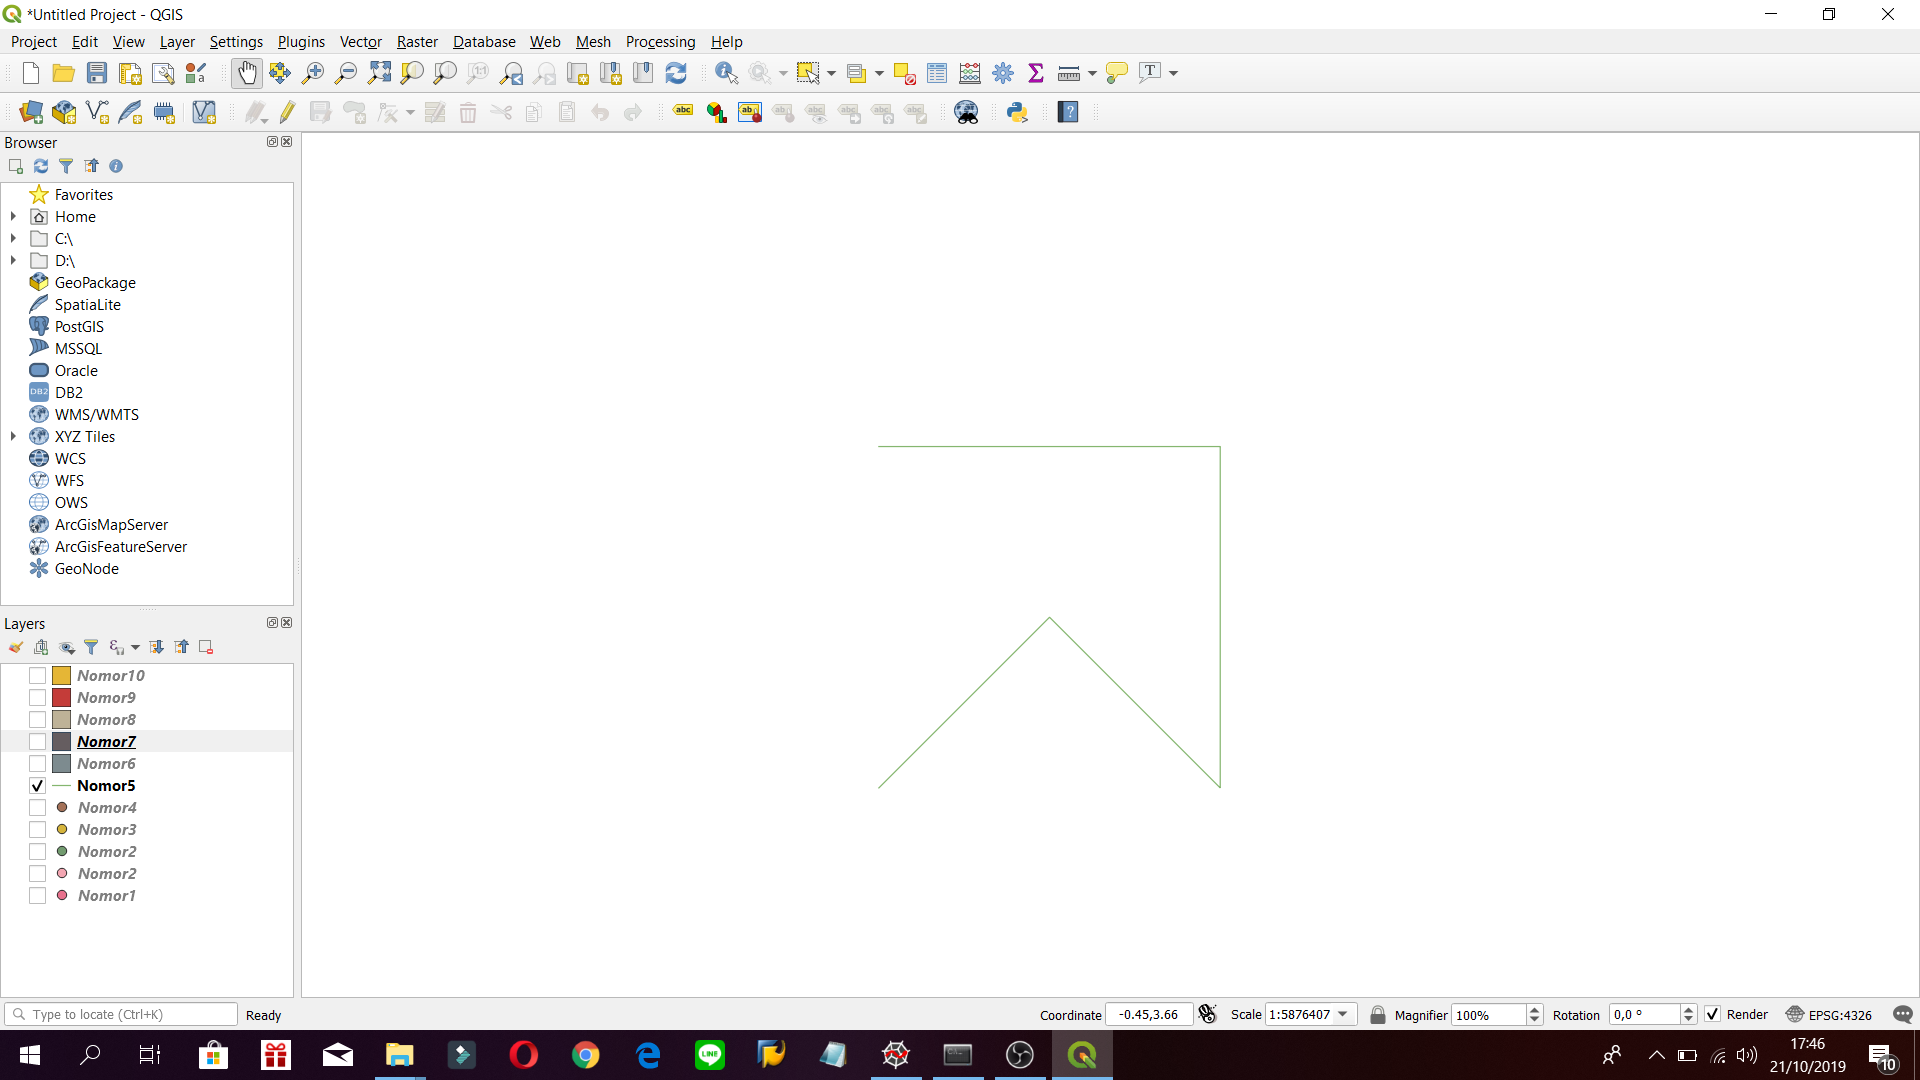
\includegraphics[width=6cm]{figures/Tugas2/1174073/No5.png}
		\centering
		\caption{PolyLine (Garis)}
	\end{figure}
	\item Nomor 6
	\lstinputlisting{src/tugas2/1174073/No6.py}
	\begin{figure}[H]
		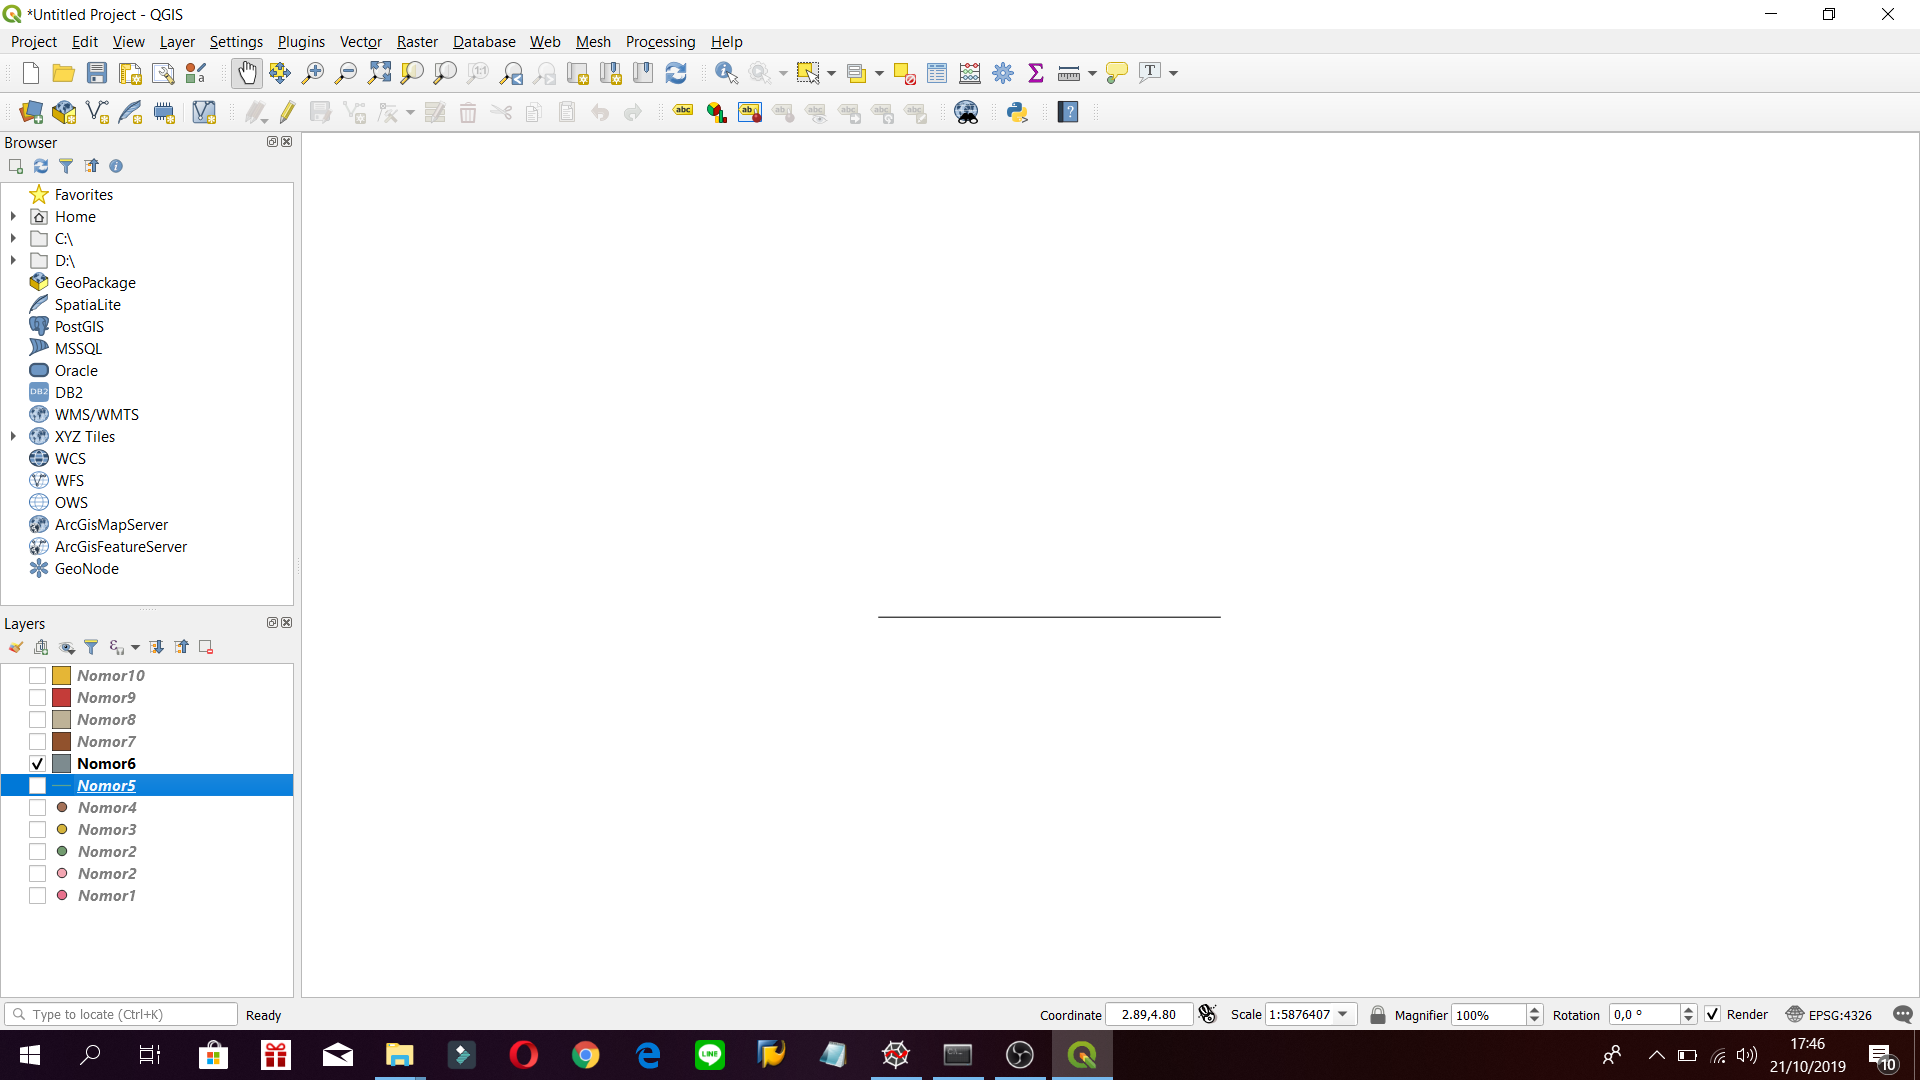
\includegraphics[width=6cm]{figures/Tugas2/1174073/No6.png}
		\centering
		\caption{Polygon (Bidang)}
	\end{figure}
	\item Nomor 7
	\lstinputlisting{src/tugas2/1174073/No7.py}
	\begin{figure}[H]
		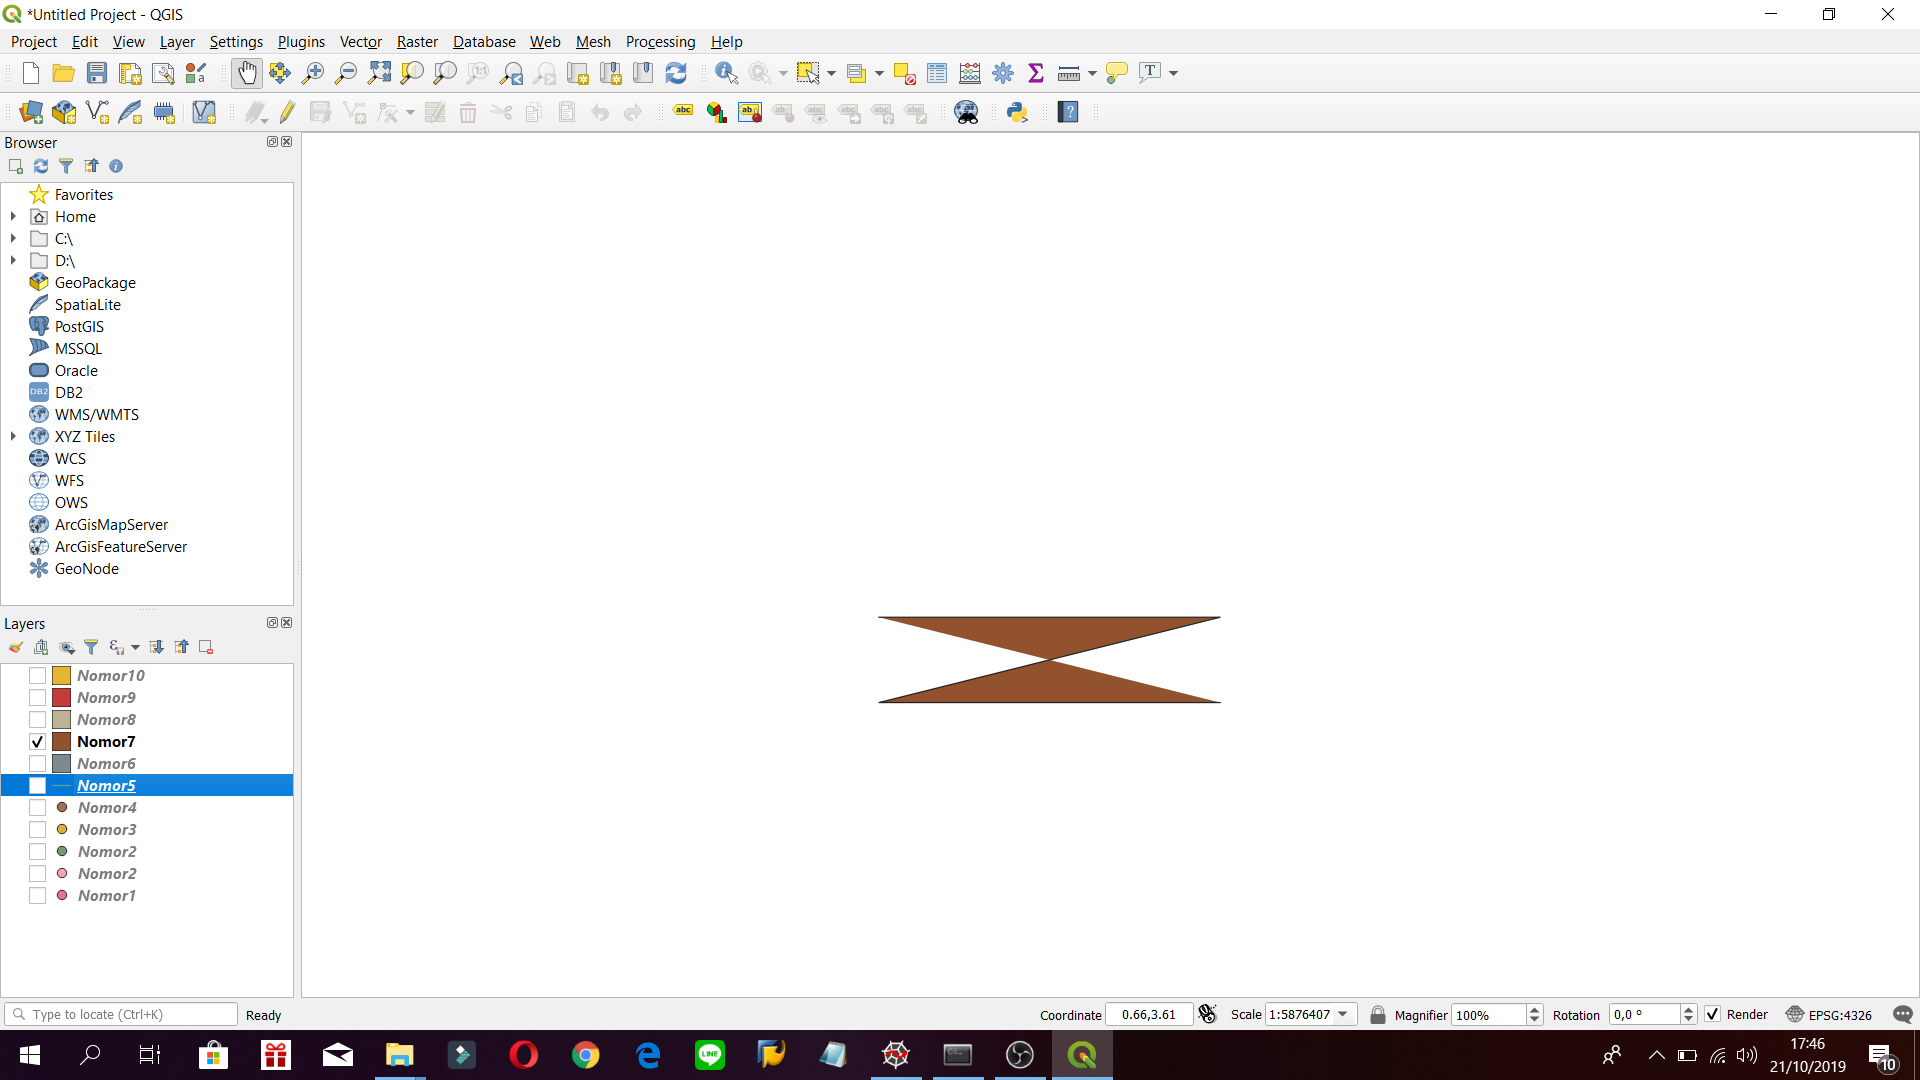
\includegraphics[width=6cm]{figures/Tugas2/1174073/No7.png}
		\centering
		\caption{Polygon (Bidang)}
	\end{figure}
	\item Nomor 8
	\lstinputlisting{src/tugas2/1174073/No8.py}
	\begin{figure}[H]
		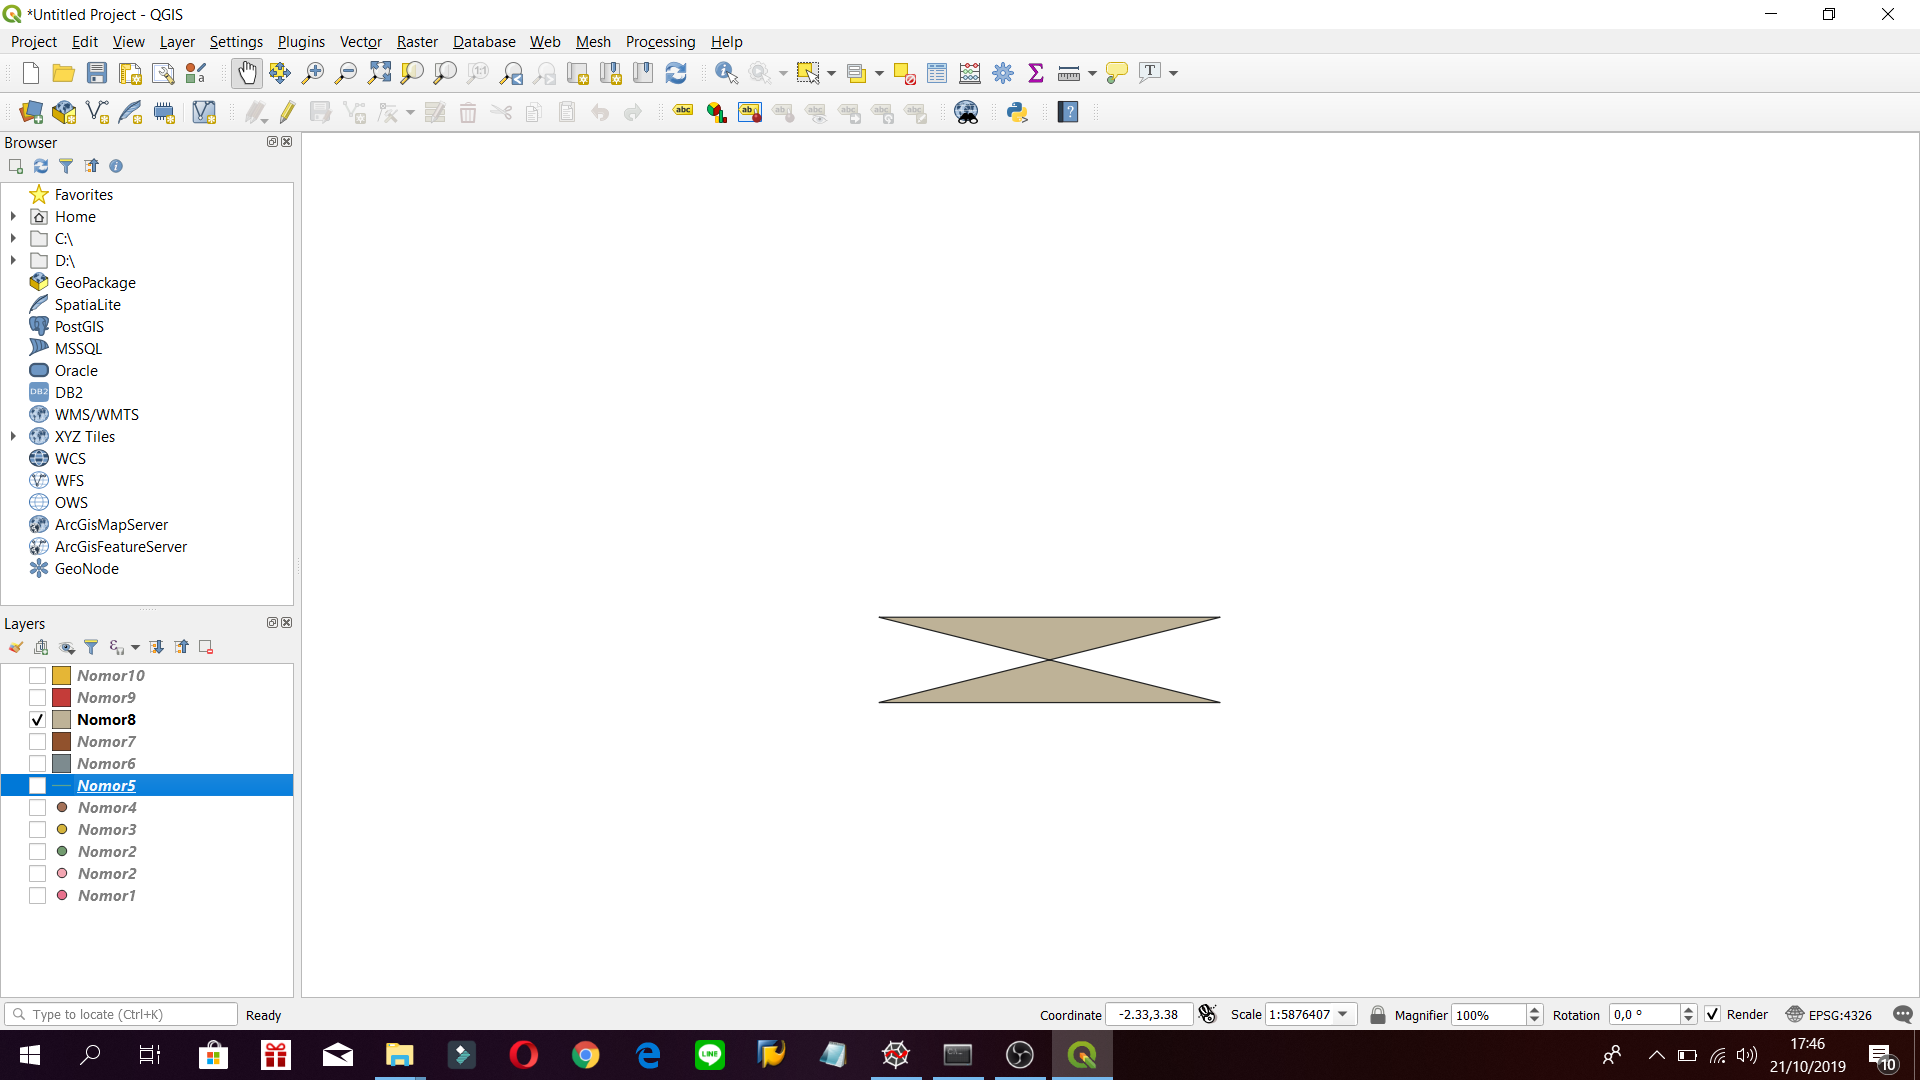
\includegraphics[width=6cm]{figures/Tugas2/1174073/No8.png}
		\centering
		\caption{Polygon (Bidang)}
	\end{figure}
	\item Nomor 9
	\lstinputlisting{src/tugas2/1174073/No9.py}
	\begin{figure}[H]
		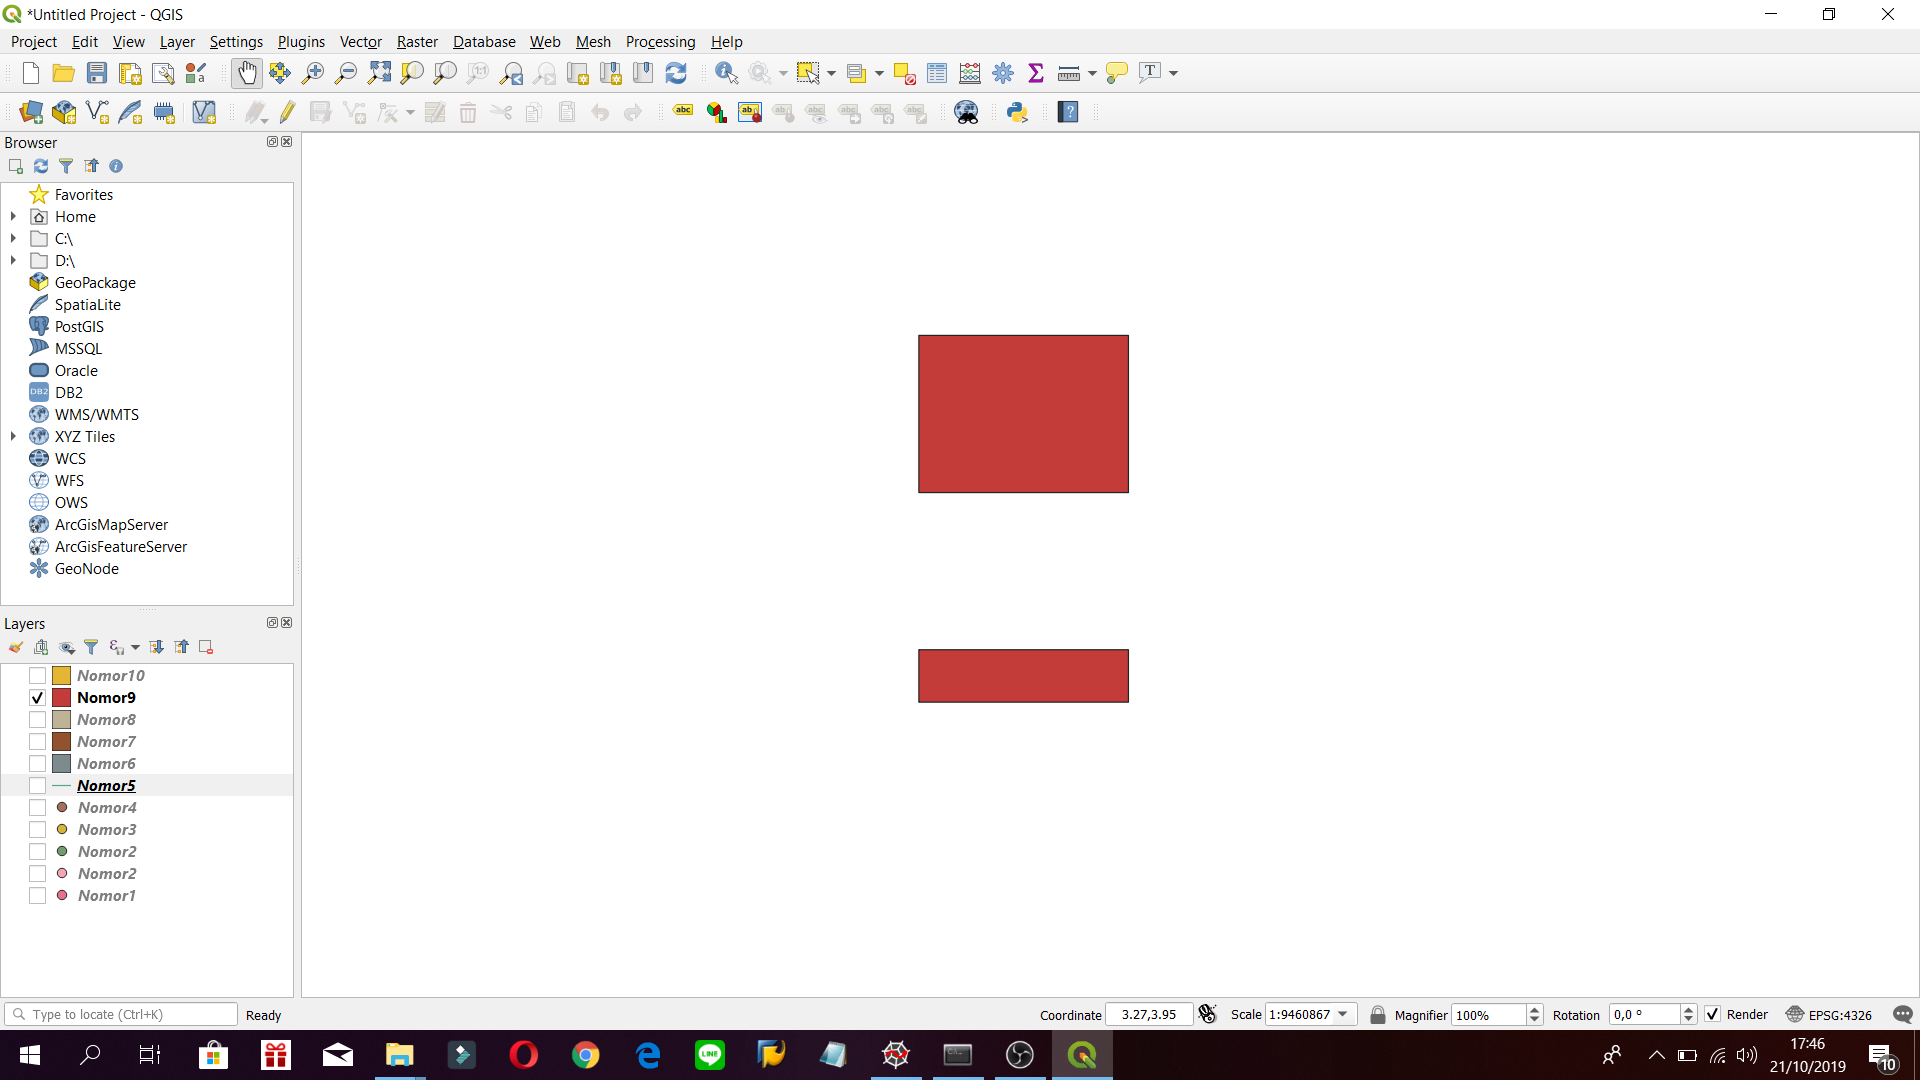
\includegraphics[width=6cm]{figures/Tugas2/1174073/No9.png}
		\centering
		\caption{Polygon (Bidang)}
	\end{figure}
	\item Nomor 10
	\lstinputlisting{src/tugas2/1174073/No10.py}
	\begin{figure}[H]
		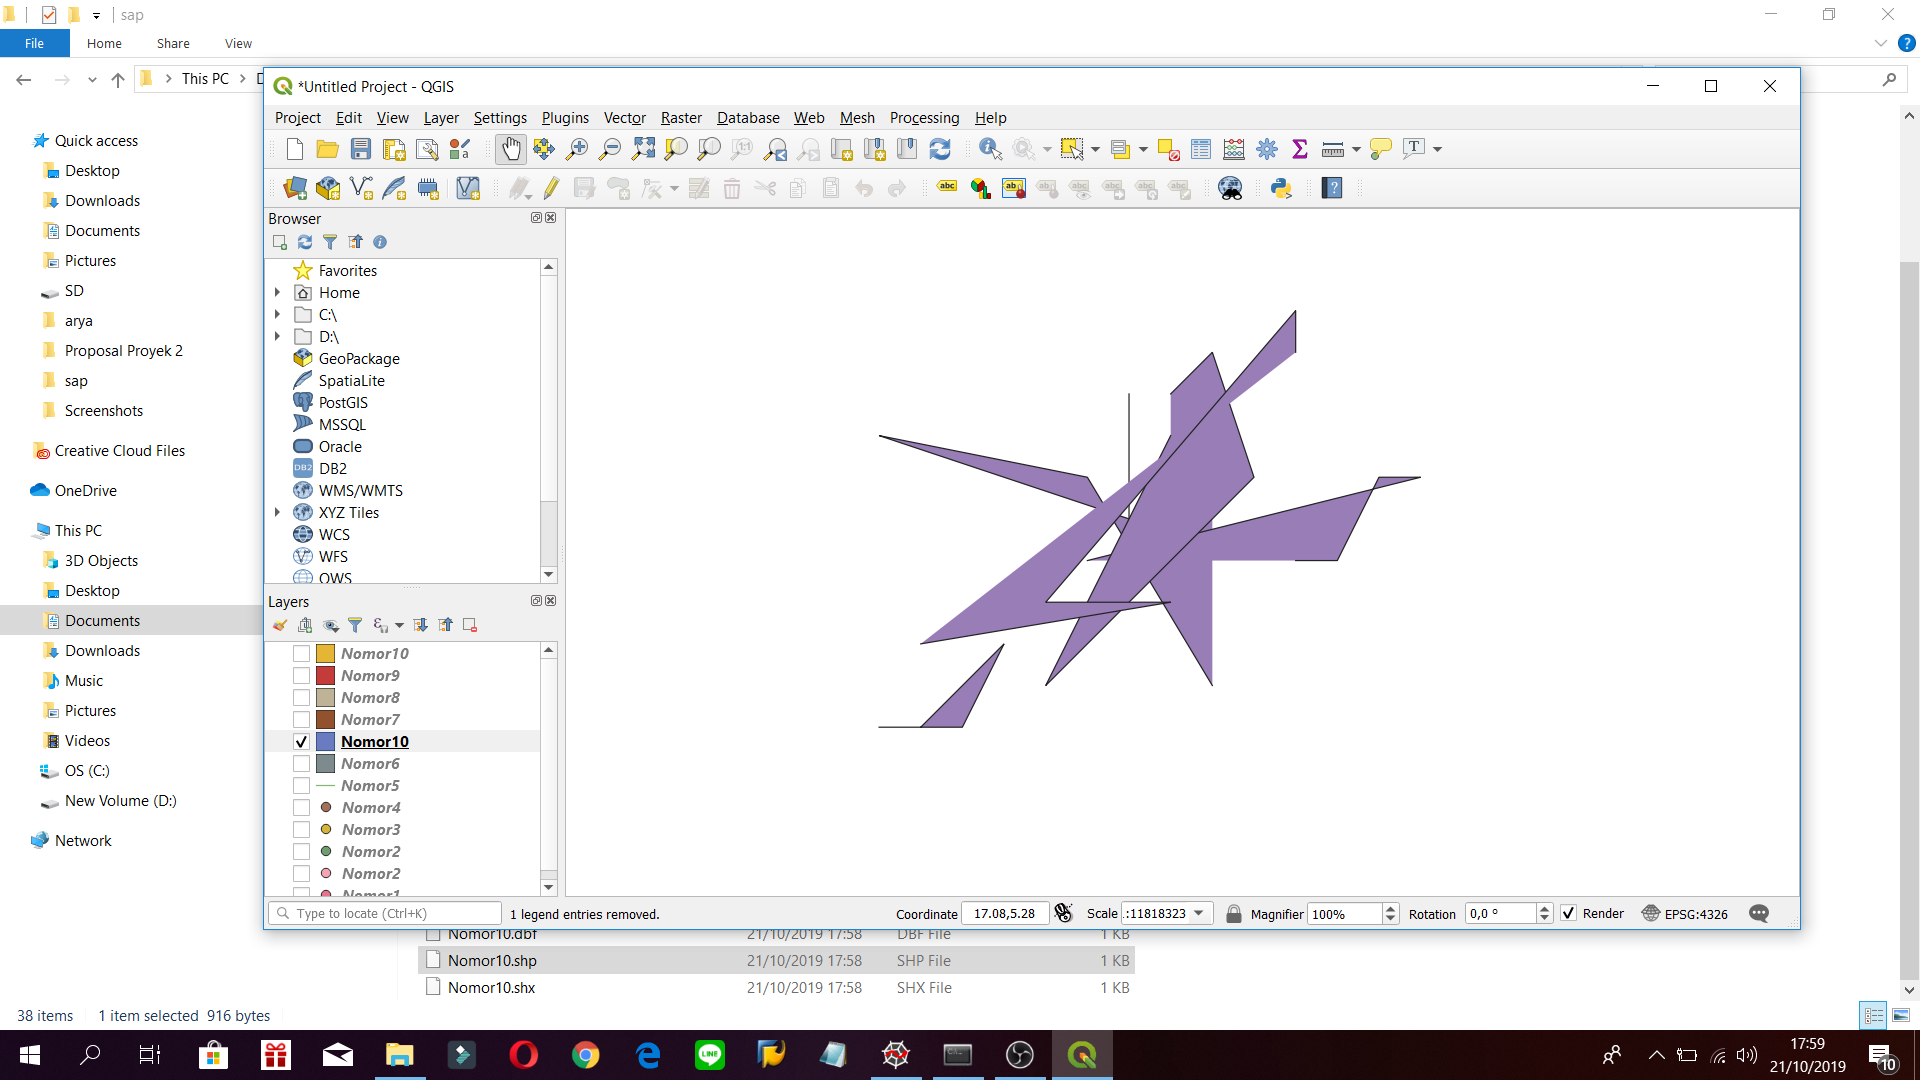
\includegraphics[width=6cm]{figures/Tugas2/1174073/No10.png}
		\centering
		\caption{Polygon, Hasil modulus dari npm saya 1174073}
	\end{figure}
\end{enumerate}
\subsection{Link}
https://youtu.be/rYMRd3M9Ahs